\documentclass[11pt]{article}
\usepackage[utf8]{inputenc}
\usepackage[russian]{babel}
\usepackage[T1]{fontenc}
\usepackage{amssymb,amsmath,clrscode,graphicx,indentfirst}

\author{Олег Смирнов}
\title{Курс kiev-clrs -- Лекция 18. Кратчайшие пути: алгоритм Беллмана-Форда, линейное программирование}
\date{18 июля 2009 г.}

\begin{document}
\maketitle
\tableofcontents
\newpage
\setlength{\parskip}{1ex plus 0.5ex minus 0.2ex}
\section{Цель лекции}
\begin{itemize}
\item Задача кратчайшего пути в графе с отрицательными дугами
\item Линейное программирование
\end{itemize}

\section{Алгоритм Беллмана-Форда}
Алгоритм решает ту же задачу, что алгоритм Дейкстры, но работает в графах с отрицательными дугами и позволяет обнаруживать отрицательные циклы. Алгоритм проще в реализации, но хуже в производительности.
\begin{codebox}
\Procname{$\proc{Bellman\_Ford}(G, w, s)$}
\li $d[s] \gets 0$
\li \For each $v \in V - \{s\}$
\li     \Do $d[v] \gets \infty$ 
    \End
\li \For $i \gets 1$ \To $|V|-1$
\li     \Do \For each $(u, v) \in E$
\li        \Do \If $d[v] > d[u] + w(u, v)$ \Comment релаксация дуги
\li            \Then $d[v] \gets d[u] + w(u, v)$
               \End
           \End
    \End
\li \For each $(u, v) \in E$ \Comment проверка наличия отрицательных циклов
\li     \Do \If $d[v] > d[u] + w(u, v)$ \Comment релаксация возможна?
\li         \Then \Return False \Comment есть отрицательный цикл
            \End
        \End
\li \Return $d$
\end{codebox}
Алгоритм вычисляет путь с кратчайшим весом $\delta(s, v)$ из истока $s \in V$ во все вершины $v \in V$. Время выполнения $T = O(V \cdot E)$ как минимум квадратично от количества вершин, если граф связный.

Для иллюстрации работы на примере нужно задать некоторый (произвольный) порядок для дуг графа:
\begin{figure}[h!]
  \centering
  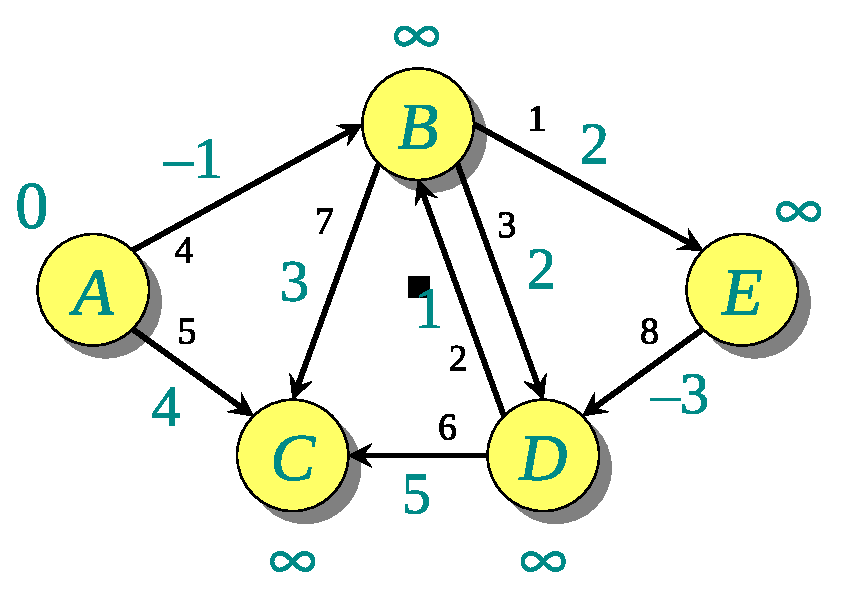
\includegraphics[width=3in]{lecture18/bellmanford1.eps}
  \caption{Шаг 1}
\end{figure}

Первая итерация цикла даст следующий результат:
\begin{center}
\begin{tabular}{|r|c|c|c|c|c|}
  \hline
      & \textbf{A} & \textbf{B} & \textbf{C} & \textbf{D} & \textbf{E} \\
  \hline
         & 0 & $\infty$ & $\infty$ & $\infty$ & $\infty$ \\
  \hline
         & 0 & -1 & $\infty$ & $\infty$ & $\infty$ \\
  \hline
         & 0 & -1 & 4 & $\infty$ & $\infty$ \\
  \hline
         & 0 & -1 & 2 & $\infty$ & $\infty$ \\
  \hline
\end{tabular}
\end{center}

На второй итерации:
\begin{center}
\begin{tabular}{|r|c|c|c|c|c|}
  \hline
      & \textbf{A} & \textbf{B} & \textbf{C} & \textbf{D} & \textbf{E} \\
  \hline
         & 0 & -1 & 2 & $\infty$ & 1 \\
  \hline
         & 0 & -1 & 2 & 1 & 1 \\
  \hline
         & 0 & -1 & 2 & -2 & 1 \\
  \hline
\end{tabular}
\end{center}

Для оптимизации алгоритм можно остановить, если на очередной итерации веса вершин не изменились. Для доказательства корректности необходимо показать, что алгоритм сходится, т.е. что за $|V|-1$ итераций будут гарантировано получены кратчайшие пути до всех вершин. Алгоритм выполняет только релаксацию, т.е. можно использовать леммы, доказанные для алгоритма Дейкстры. 

У алгоритма Беллмана-Форда есть интересная особенность: его можно выполнять на многопроцессорной системе. Шаг релаксации можно выполнять независимо на каждом из узлов.

Лемма корректности: если в графе $G=(V, E)$ нет циклов с отрицательным весом, тогда алгоритм Беллмана-Форда завершается с $d[v] = \delta(s, v)$.

Необходимо доказать, что $d[v] \gets \delta(s, v)$ в какой-то момент времени, т.к. по лемме о релаксации, $d[v]$ может только уменьшаться и никогда не станет меньше необходимого значения.

Пусть $p = v_0 \rightarrow v_1 \rightarrow \ldots \rightarrow v_k$, где $v_0 = s$, $v_k = v$ -- кратчайший путь из $s$ в $v$, который содержит минимальное количество вершин. Тогда $p$ -- это простой путь, т.е. на нём нет повторяющихся вершин.

По лемме об оптимальной подструктуре: $\delta(s, v_i) = \delta(s, v_{i-1}) + w(v_{i-1}, v_i))$.

Для доказательства по индукции необходимо проверить базовый случай: $d[v_0] = 0 = \delta(s, v_0) = \delta(s, s)$. База индукции выполняется, т.к. в графе нет отрицательных циклов.

Пусть $d[v_j] = \delta(s, v_j)$ после $j$-го шага итерации алгоритма, где $j < i$. Тогда на $i$-м шаге после релаксации дуги $(v_{i-1}, v_i)$, $d[v_i]$ станет равным $\delta(s, v_{i-1}) + w(v_{i-1}, v_i) = \delta(s, v_i)$. Таким образом, после $k$ итераций будет получено правильное значение пути для $d[k]$. Так как количество вершин в простом пути в графе не превышает $|V|-1$, такое же количество итераций необходимо, чтоб получить все пути.

Следствие: если алгоритм Беллмана-Форда не сошелся после $|V|-1$ итераций (т.е. дальнейшие релаксации возможны), то в графе есть циклы с отрицательным весом.

\section{Линейное программирование}
Дана матрица $A$ размера $m \times n$ и $m$-элементный вектор $b$ и $n$-элементный вектор $c$. Найти вектор $x$ размера $n$, такой, что $c^{T} \cdot x$ (целевая функция) максимально и $A\cdot x \leqslant b$ (выполняются ограничения), если такой вектор существует.

Существует много методов решения задачи линейного программирования. Например:
\begin{itemize}
\item симплекс-метод (экспоненциальное время в худшем случае)
\item метод эллипсоидов (полиноминальное время) 
\item метод внутренней точки
\end{itemize}

Задача разностных ограничений является частным случаем задачи линейного программирования со следующими вариациями:
\begin{itemize}
\item ответ -- любое допустимое решение (нет ограничения целевой функции)
\item в каждой строке матрицы ограничений $A$ один элемент $1$, один $-1$, остальные -- нули
\end{itemize}
Т.е. каждое ограничение имеет форму:
\begin{equation}
  x_j - x_i \leqslant w_{i j}
  \label{eq:constr}
\end{equation}
Пример задачи:
\begin{align*}
  x_1 - x_2 \leqslant 3 \\
  x_2 - x_3 \leqslant -2 \\
  x_1 - x_3 \leqslant 2  
\end{align*}
Ответ:
\begin{align*}
  x_1 = 3 \\
  x_2 = 0 \\
  x_3 = 2 
\end{align*}
Задачу разностных ограничений можно представить в виде графа (ограничений) $G=(V, E)$, где $|V|=n$, $|E|=m$. Каждое неравенство вида $x_j - x_i \leqslant w_{i j}$ представляется в виде дуги между вершинами:
\begin{figure}[h!]
  \centering
  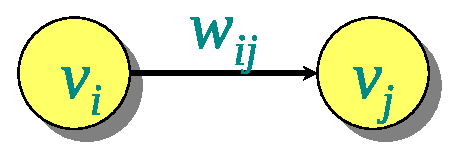
\includegraphics[width=1.5in]{lecture18/edge.eps}
  \caption{Дуга ограничений}
\end{figure}
Связь между графом и ограничениями можно увидеть, переписав неравенство (\ref{eq:constr}) в виде:
\begin{align*}
  x_j \leqslant x_i + w_{i j} \\
  d[j] \leqslant d[i] + w(i, j)
\end{align*}

Теорема: если в графе ограничений есть циклы отрицательного веса, то соответствующая задача разностных ограничений не имеет допустимого решения.

Доказательство: пусть $v_1 \rightarrow v_2 \rightarrow \ldots \rightarrow v_k \rightarrow v_1$ -- путь весом строго меньше нуля. Тогда ему соответствуют следующие ограничения:
\begin{align*}
  x_2 - x_1 \leqslant w_{12} \\
  x_3 - x_2 \leqslant w_{23} \\
  \ldots \\
  x_k - x_{k-1} \leqslant w_{k-1 k} \\
  x_1 - x_k \leqslant w_{k 1}
\end{align*}
Если сложить обе неравенства, получим:
\begin{align*}
  0 \leqslant w(\text{пути}) < 0
\end{align*}
Т.о. система неравенств не имеет допустимого решения.

Теорема: если в графе $G$ нет циклов отрицательного веса, то у задачи разностных ограничений есть решение.

Доказательство: добавить в граф $G$ вершину $s$ соединенную с каждой вершиной $v \in V$ дугой веса $0$.
\begin{figure}[h!]
  \centering
  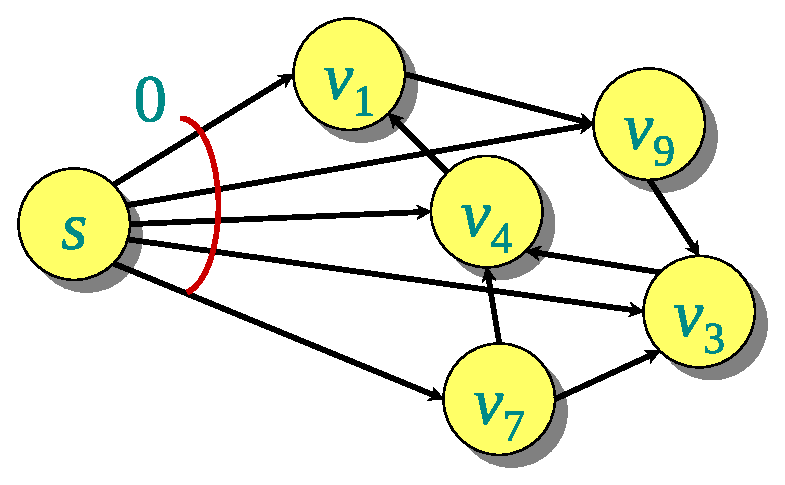
\includegraphics[width=3in]{lecture18/graph1.eps}
  \caption{Граф ограничение}
\end{figure}
В этом графе нет циклов отрицательного веса и есть кратчайшие пути из $s$ в каждую вершину весом не более $0$. Обозначим $x_i = \delta(s, v_i)$.

Неравенство $x_j - x_i \leqslant w_{i j}$ эквивалентно
\begin{align*}
   \delta(s, v_i) - \delta(s, v_j) \leqslant w_{i j} \iff \\
   \iff \delta(s, v_i) \leqslant \delta(s, v_j) + w_{i j}
\end{align*}
Последнее неравенство истино, т.к. это неравенство треугольника. Следовательно исходное неравенство также выполняется.

Таким образом, задачу разностных ограничений из $m$ неравенств с $n$ переменными можно преобразовать в граф, а затем решить с помощью алгоритма Беллмана-Форда за время $T = O(m n)$.

\section{Заключительные замечания}

Алгоритм Беллмана-Форда используется в протоколах маршрутизации семейста ``distance-vector routing'', например в протоколе RIP версий 1 и 2.

\end{document}
